\documentclass{LTHthesis}
\usepackage[T1]{fontenc}
\usepackage[utf8]{inputenc}  %% Comment if you are not using utf8
\usepackage{mathptmx, helvet}
\usepackage{graphicx}
\usepackage[colorinlistoftodos]{todonotes}

%To write pseudo code
\usepackage[chapter]{algorithm}
\usepackage{algpseudocode}
\MakeRobust{\Call}
\newcommand{\inp}[1]{\hspace*{\algorithmicindent}\textbf{Input:} #1\\}
\newcommand{\outp}[1]{\hspace*{\algorithmicindent}\textbf{Output:} #1\\}
\let\oldforall\forall
\renewcommand{\forall}{\hspace*{2mm}\oldforall\hspace*{1mm}}
\let\oldexists\exists
\renewcommand{\exists}{\hspace*{2mm}\oldexists\hspace*{1mm}}
\newcommand{\emptyvec}{[\hspace*{1mm}]}

\usepackage[super]{nth}

%Image inputs
\newcommand{\proofimage}[2]{\begin{figure}[H]\makebox[\textwidth][c]{\includegraphics[width=0.9\textwidth]{#1}}\caption{#2}\end{figure}}
\newcommand{\popimage}[1]{\begin{figure}[H]\makebox[\textwidth][c]{\includegraphics[width=1.2\textwidth]{#1}}\end{figure}}

%Input code
\usepackage{minted}
\newcommand{\codep}[1]{\inputminted[fontsize=\large,tabsize=1,baselinestretch=1]{py}{code/#1}}

%For tables
\usepackage{array}
\newcolumntype{L}[1]{>{\raggedright\let\newline\\\arraybackslash\hspace{0pt}}m{#1}}
\newcolumntype{C}[1]{>{\centering\let\newline\\\arraybackslash\hspace{0pt}}m{#1}}
\newcolumntype{R}[1]{>{\raggedleft\let\newline\\\arraybackslash\hspace{0pt}}m{#1}}
\let\oldhline\hline
\renewcommand{\hline}{\oldhline\vspace*{6mm}}

%\newcommand{\vect}[1]{\boldsymbol{#1}}
%Bold vector: \vec{x}
%\usepackage{amsbsy}
\renewcommand{\vec}[1]{\mathbf{#1}}
%BigO
%\renewcommand{\bigO}[0]{\mathcal{O}}

%Short cuts
\newcommand{\reference}[1]{[\ref{Ref: #1}]}
%\newcommand{\WZ}{Wilf-Zeilberger's method}

%To get numbered subsections
\setcounter{secnumdepth}{5}

%Setting paragraph indent and skips
\usepackage{siunitx}
\setlength{\parindent}{0pt}
\setlength{\parskip}{10pt}
\setlength{\fboxsep}{.5\fboxsep}

%Theorems
\theoremstyle{definition}
\newtheorem{theorem}{Theorem}[chapter]
\newtheorem{example}[theorem]{Example}
\newtheorem*{solution}{Solution}
\newtheorem{lemma}[theorem]{Lemma}
\newtheorem{definition}[theorem]{Definition}
\newtheorem*{remark}{Remark}


%\addbibresource{mybib.bib}  %%  Comment if you don't want to use bibtex.

\begin{document}
\begin{titlepages}
\author{Lars Åström}
\title{Polynomial Computer Algebra and implementation of Wilf-Zeilberger's method}
\year{2019}
\month{December}
\TFRT{TODO}  %%  You will get the number from the department.
\printer{Media-Tryck}  %% Probably. You may get other information from the department.
\end{titlepages}
\chapter*{Abstract}
The purpose of the thesis is to get a better understanding of computer algebra in general, and polynomial computer algebra in particular. This is done by implementing a library for a polynomials and methods that are needed to be able to perform operations on the polynomials. Then this library is used to implement Wilf-Zeilberger's method, which is a method that can be used to prove certain combinatorial identities involving summation. The thesis consists mostly of three parts; theory, implementation and examples. In the theory section, all the theoretical results used in the project are presented. The implementation section then treats the difficulties arising when turning theory into practice, and focuses in particular on when theoretically easy methods and concepts become much more challenging in implementation. The program that is developed seems to work well, both on examples that were used throughout the project as testing and on validation examples that were found after all the implementation was done. This means that the program can solve and produce a paper proving that identities indeed are true. Therefore the thesis shows one example of how automated proofs can be generated, but mostly the thesis highlights the difficulties arising in computer algebra while implementing the specific example of Wilf-Zeilberger's method.


\chapter*{Abstrakt}
En kort sammanfattning på ungefär 250 ord. Observera att denna är obligatorisk och ska skrivas på engelska och gärna också på svenska.


\chapter*{Preface}
The thesis has been written in Lund during September-December 2019, as a master's thesis in the program Engineering in Mathematics. The idea of the thesis came from my supervisor, professor Victor Ufnarovski, who presented ten different, all very interesting problem formulations for a master thesis, only a few days after I asked if he had any ideas that we could do as a master's thesis.

Firstly, I would like to thank my supervisor Victor Ufnarovski, who has not only been of great help during the thesis work, but also previously in my life as coach in the international mathematics olympiad. There I got help both to become better at mathematics, but also in other aspects with continuous positive feedback.

Secondly, I would like to thank my family and friends, who have supported me both while writing my thesis and previously in my studies and in my life.


\tableofcontents

\chapter{Introduction}\label{Ch: Introduction}
In the thesis computer algebra is investigated and a library for manipulating and working with polynomials is produced. Then this package is used to implement \WZ, which is a method to prove identities involving (infinite) summation. Although there already are toolboxes available in several different software languages that handles polynomials we will develope a new system, in order to experience implementation pitfalls and difficulties first hand.

Computer algebra has been developed during the second half of the \nth{20} century. Martinus Veltman won the Nobel prize in physics 1999 due to his work with developing a computer algebraic software for particle physics. The first working version dates back to the 1960s. \reference{veltman} This was one example of an early computer algebraic system.

Computer algebraic systems are used to automize manipulation of mathematical expressions that are similar to traditional pen and paper calculations. The advantage of computer algebra is that the power of a computer is used, meaning that computations can be performed extremely fast and with improved computational power the possibilities are neverending. This is the reason computer algebra is growing as a field, and why it is both important and interesting to investigate.

Before starting this thesis I did not know much about computer algebra. Although it is a big part of almost all tools that have been used during courses in my program at LTH (such as MATLAB and Maple), I have never given the details of how implementation is done much thought. Therefore this thesis has given me the opportunity to investigate the basics of computer algebra, while providing an open source implementation of \WZ.

The goal of the thesis is to, by implementing a library for polynomial computer algebra, implement an automatic solver which can prove identities using \WZ. Furthermore the goal is to get a deeper understanding of implementation difficulties in computer algebra by implementing everything, and the implementation should rather be simple and easy to understand than complicated but more efficient computationally.

\todo[inline]{change all WZ to \WZ.}


\chapter{Background}\label{Ch: Background}
Computer algebra, also called symbolic computation or algebraic computation, is the study of algorithms and software for simplifying and manipulating mathematical expressions. Computer algebra has many applications, is a part of many different mathematical languages, such as Maple and Mathematica, and is used widely in many mathematical and engineering applications, such as physics and cryptography.\reference{maple}\reference{computeralgebra}

In combinatorics binomial coefficients are constantly used for counting different things. Also the sum of binomial coefficients are often of interest in solving the theoretical questions in combinatorics and similar fields. Some combinatorial identities have beautiful and simple proofs using combinatorial arguments while others require long and complicated proofs. Therefore Wilf-Zeilberger's method comes in handy, to automize the proof procedure.

In the thesis Wilf-Zeilberger's method will be used and implemented, which is a method to prove the correctness of an (infinite) sum. One example where it can be used is to prove
\begin{equation}\label{Eq: Background}
  \sum_{k=0}^n (-1)^k\binom{n}{k}\binom{2k}{k}4^{n-k}=\binom{2n}{n}.
\end{equation}
Here we see that we have a finite sum, but it can also be seen as an infinite sum from $-\infty$ to $\infty$ too, if we define $\binom{n}{a}=0$, when $a<0$ or $a>n$.

The steps of the method will of course be shown in chapter \ref{Ch: Theory}, but the general idea is to change our addends in the sum to something that telescopes. After this is done, proving the identity gets reduced to prove the identity for a single $n$. As we see in equation \ref{Eq: Background} this is quite easy to prove for some $n$, for instance $n=0$. Although it is not always easy to prove the identity for some $n$, it is usually the case.

Wilf-Zeilberger's method itself is not a very new method, it dates back to 1990.\reference{wz} Even implementations of the method in computer algebraic softwares is not very new, for instance an implementation of the method in Mathematica was published in 1994.\reference{mathematica} The contribution of this thesis is therefore not an implementation of something that has not been implemented before, but rather an open source version of it. Furthermore, as stated in chapter \ref{Ch: Introduction}, a large part of the goal is to get a better understanding of computer algebra.


\chapter{Theory}\label{Ch: Theory}
\section{Polynomials}
In the thesis we are continuously discussing polynomials. We are always using polynomials with integer coefficients -- which we also generalize to include rational coefficients by looking at fractions of polynomials with integer coefficients. Therefore, from now on whenever we talk about polynomials they are assumed to have integer coefficients as long as otherwise is not stated.[\ref{Ref: gosper}]\todo{This is an example, remove when adding references.}

We will now have a discussion on what operations we want to be able to perform on the polynomials both theoreticly and partly implementation wise. Therefore there will not be a specific subchapter regarding polynomials later on in chapter \ref{Ch: Implementation}. But first we need to describe how a polynomial can be implemented and stored in the code -- and this is how it was implemented in this thesis.

A polynomial, say $p(n)$, can be seen as a list of coefficients $[a_0,a_1,\ldots,a_d]$. This represents the polynomial
\begin{equation}\label{Eq: Theory,polynomials,general polynomial}
  p(n) = a_0+a_1 n + \ldots + a_d n^d.
\end{equation}
This is fairly simple if the polynomial only has one variable. As soon as we introduce polynomials with more than one variable -- which is the case in all examples where Wilf-Zeilbergers method is used -- it gets a bit more complicated. The way we will visualize polynomials of more than one variable is to try to keep the very same structure as in \ref{Eq: Theory,polynomials,general polynomial}, namely we store a polynomial $p(n)$ as a list of coefficients $[a_0,a_1,\ldots,a_d]$, but instead of having $a_i$ just representing integers they are instead themselves polynomials. In order to show how this can be done, lets show an example.
\begin{example}\label{Ex: polynomial, recursive}
  Lets look at the polynomial
  \begin{equation*}
    \begin{split}
      p(k,m,n) = &1+3n+2n^2-m-2mn-2mn^2+3m^2+3m^2n+3m^2n^2+\\
      &3k-3kn+2kn^2+km-2kmn-km^2+2k^2-k^2n-k^2n^2+\\
      &3k^2m-3k^2mn-2k^2mn^2-3k^2m^2-k^2m^2n-3k^2m^2n^2.
    \end{split}
  \end{equation*}
  This will be stored as
  \begin{equation*}
    \begin{split}
      p(k,m,n) = & -((3k^2+3k-3)m^2-(2k+1)m-(3k^2-k+3))n^2+\\
      &((k^2-1)m^2-(k^2-2k+2)m-(2k+2))n+\\
      &((2k^2+2)m^2+(2k-1)m+(k^2-k-3))
    \end{split}
  \end{equation*}
  Note that this can be written as
  \begin{equation*}
    p(k,m,n) = p_2(k,m)n^2+p_1(k,m)n+p_0,
  \end{equation*}
  where
  \begin{equation*}
    \begin{split}
      p_0(k,m) &= ((2k^2+2)m^2+(2k-1)m+(k^2-k-3))\\
      p_1(k,m) &= ((k^2-1)m^2-(k^2-2k+2)m-(2k+2))\\
      p_2(k,m) &= -((3k^2+3k-3)m^2-(2k+1)m-(3k^2-k+3)).
    \end{split}
  \end{equation*}
  Now since our definition of polynomials is recursive, each of $p_0(k,m),p_1(k,m),p_2(k,m)$ is written as $q_2(k)m^2+q_1(k)m+q_0(k)$ for polynomials $q_0,q_1,q_2$. For instance for $p_1$ we have
  \begin{equation*}
    p_1(k,m) = q_2(k)m^2+q_1(k)m+q_0(k),
  \end{equation*}
  where
  \begin{equation*}
    \begin{split}
      q_0(k) & = -(2k+2) \\
      q_1(k) & = -(k^2-2k+2) \\
      q_2(k) & = (k^2-1)
    \end{split}
  \end{equation*}
  Lastly we have the polynomials $q_0,q_1,q_2$ which have integers as coefficients.
\end{example}
As we saw in example \ref{Ex: polynomial, recursive} we define all polynomials as in equation \ref{Eq: Theory,polynomials,general polynomial} where the coefficients $a_i$ are polynomials or integers, where it is only integers in the base case.

Note that in this case we wrote the polynomial with $n$ ''outmost'' in the representation of $p$. There was no specific reason for this, and the choice is not very important when only looking at one polynomial at a time. When we are using several polynomials at the same time, for instance if we want to add two polynomials, the structure is crucial. Therefore we will define some concepts regarding the representation of a polynomial.

\begin{definition}
  A polynomial $p$ is said to have the variable order $\vec{x}=(x_1,x_2,\ldots,x_m)$ if it is stored as
  \begin{equation}
    p(\vec{x}) = \sum_{i_1=0}^{d_1}\Bigg(\sum_{i_2=0}^{d_2}\Big(\sum_{i_3=0}^{d_3}\ldots\Big)x_2^{i_2}\Bigg)x_1^{i_1}.
  \end{equation}
  Note that the same polynomial can be expressed in various different ways, and we say that two variable orders, $\vec{x}$ and $\vec{y}$, are different if $|\vec{x}|\neq|\vec{y}|$ (where $|\vec{z}|$ denotes the length of the vector $\vec{z}$) or there exist an integer $i$ such that $x_i\neq y_i$.
\end{definition}
\begin{remark}
  If the polynomial $p$ has variable order $\vec{x}=(x_1,x_2,\ldots,x_m)$, then the coefficients of $p$ have variable order $\vec{x^\prime}=(x_2,\ldots,x_m)$.
\end{remark}
\begin{remark}
  Note that if the polynomial $p$ has variable order $\vec{x}$ such that $|\vec{x}|=1$, then the coefficients of $p$ are integers.
\end{remark}

Here we can note that $d_i$ is the degree of $p$ with respect to $x_i$. Furthermore we note that we can express a polynomial $p$ with the variable order $\vec{x}=(x_1,\ldots,x_m)$ even though $p$ does not have all the variables $x_j$ in its expression. If $p$ does not depend on $x_j$ that will be seen in that $d_j=0$. A polynomial $p$ cannot, however, be expressed with the variable order $\vec{x}$ if not all its variables are in $\vec{x}$. A last note is that we can convert a polynomial $p$ with variable order $\vec{x}$ to any variable order $\vec{y}$ as long as $x_i\in\vec{y} \forall x_i\in\vec{x}$.

There are of course many operations that are needed when operating with polynomials; addition, negate, subtraction, multiplication, division, modulo, gcd (greatest common divisor), checking for equality, finding roots and evaluating at a point. In the implementation all of them are defined recursively. We will show how this is done for all the most straight forward operations here, while the more complicated operations -- division, modulo and gcd -- are described later in section \ref{Ch: div,mod,gcd}.

First we define how we write that a polynomial is constructed:
\begin{definition}
  When we construct a polynomial $p$ of a variable $x$ then we write this as
  \begin{equation}
    p = polynomial(\vec{a},"x"),
  \end{equation}
  where $\vec{a}=(a_0,a_1,\ldots,a_d)$. This means that
  \begin{equation}
    p(x) = a_0 + a_1 x + \ldots + a_d x^d.
  \end{equation}
  Note that we have not specified what $a_i$ are; they can be either integers or polynomials -- but if they are polynomials they have to have the same variable order. Also note that once we have the polynomial $p$ we will use the notation $p[i]$ to reference the $i$-th variable, namely $a_i$. If we reference $p[j]$ where $j\ge d$, then this is defined as $p[j]=0 \forall j\ge d$.
\end{definition}

We also define the degree of a polynomial:
\begin{definition}
  Let the polynomial $p$ have variable order $\vec{x}=(x_1,\ldots,x_m)$. Then we define the degree of $p$, denoted $deg(p)$, as the largest exponent of $x_1$ in the expression for $p$.
\end{definition}

For all the operations we will use two polynomials $f$ and $g$. These are polynomials with the variable order $\vec{x}$. We will now provide procedures that show how all the previously mentioned operations should work. Note that the procedures are assuming that the polynomials have the same variable order, if this is not the case then the polynomials first are converted into a common variable order.

All the procedures try to follow the same structure, which is quite recursive. All procedures have a base case, usually when $|\vec{x}|=1$, and in all other cases recursive calls are made. A note to be made here is that recursive calls are not computationally heavy in theory but might take time if many are made, especially if the depth is large, in practice. In this thesis however, the depth is very small -- usually less than 5 -- since the depth comes from the number of variables in the polynomials. Therefore the recursion is not expected to cause any problems computationally.

\begin{algorithm}[H]
  \caption{Addition}
  \inp{Polynomials $f$ and $g$, with variable order $\vec{x}$}
  \outp{Polynomial $h$ such that $h=f+g$}
  \begin{algorithmic}[1]
    \Procedure{Add}{$f,g$}
      \State $\vec{a}\gets \emptyvec$
      \For{$i\gets 0,\ldots,max(deg(f),deg(g))$}
        \If{$|\vec{x}|=1$}
          \State $\vec{a}[i]\gets f[i]+g[i]$
        \Else
          \State $\vec{a}[i]\gets$ \Call{Add}{$f[i],g[i]$}
        \EndIf
      \EndFor
      \State \Return $polynomial(\vec{a},\vec{x}[0])$
    \EndProcedure
  \end{algorithmic}
\end{algorithm}

\begin{algorithm}[H]
  \caption{Negatation}
  \inp{Polynomial $f$ with variable order $\vec{x}$}
  \outp{Polynomial $h$ such that $h=-f$}
  \begin{algorithmic}[1]
    \Procedure{Negate}{$f$}
      \State $\vec{a}\gets \emptyvec$
      \For{$i\gets 0,\ldots,deg(f)$}
        \If{$|\vec{x}|=1$}
          \State $\vec{a}[i]\gets -f[i]$
        \Else
          \State $\vec{a}[i]\gets$ \Call{Negate}{$f[i]$}
        \EndIf
      \EndFor
      \State \Return $polynomial(\vec{a},\vec{x}[0])$
    \EndProcedure
  \end{algorithmic}
\end{algorithm}

\begin{algorithm}[H]
  \caption{Subtraction}
  \inp{Polynomials $f$ and $g$, with variable order $\vec{x}$}
  \outp{Polynomial $h$ such that $h=f-g$}
  \begin{algorithmic}[1]
    \Procedure{Subtract}{$f,g$}
      \State $g^\prime\gets$ \Call{Negate}{$g$}
      \State \Return \Call{Add}{$f,g^\prime$}
    \EndProcedure
  \end{algorithmic}
\end{algorithm}

\begin{algorithm}[H]
  \caption{Multiplication}
  \inp{Polynomials $f$ and $g$, with variable order $\vec{x}$}
  \outp{Polynomial $h$ such that $h=f\cdot g$}
  \begin{algorithmic}[1]
    \Procedure{Multiply}{$f,g$}
      \State $\vec{a}\gets \emptyvec$
      \For{$i\gets 0,\ldots,deg(f)+deg(g)$}
        \State $\vec{a}[i]\gets 0$
      \EndFor
      \For{$i\gets 0,\ldots,deg(f)$}
        \For{$j\gets 0,\ldots,deg(g)$}
          \If{$|\vec{x}|=1$}
            \State $\vec{a}[i+j]\gets \vec{a}[i+j] + f[i]\cdot g[j]$
          \Else
            \State $y_{i,j}\gets$ \Call{Multiply}{$f[i],g[j]$}
            \State $\vec{a}[i+j]\gets$ \Call{Add}{$\vec{a}[i+j],y_{i,j}$}
          \EndIf
        \EndFor
      \EndFor
      \State \Return $polynomial(\vec{a},\vec{x}[0])$
    \EndProcedure
  \end{algorithmic}
\end{algorithm}

\begin{algorithm}[H]
  \caption{Equality}
  \inp{Polynomials $f$ and $g$, with variable order $\vec{x}$}
  \outp{$True$ if $f$ and $g$ are equal, otherwise $False$}
  \begin{algorithmic}[1]
    \Procedure{Equals}{$f,g$}
      \If{$deg(f)\neq deg(g)$}
        \State \Return $False$
      \EndIf
      \For{$i\gets 0,\ldots,deg(f)$}
        \If{$|\vec{x}|=1$ AND $f[i]\neq g[i]$}
          \State \Return $False$
        \ElsIf{$|\vec{x}|>1$ AND $not$ \Call{Equals}{$f[i],g[i]$}}
          \State \Return $False$
        \EndIf
      \EndFor
      \State \Return $True$
    \EndProcedure
  \end{algorithmic}
\end{algorithm}

\begin{algorithm}[H]
  \caption{Evaluating at a point}
  \inp{Polynomials $f$, with variable order $\vec{x}$, variable $v\in\vec{x}$ and value $y$}
  \outp{Polynomial $h$ that is $f$ evaluated at $v=y$}
  \begin{algorithmic}[1]
    \Procedure{Evaluate}{$f,v,y$}
      \If{$\vec{x}[0]=v$}
        \State $g\gets f[0]$
        \For{$i\gets 1,\ldots,deg(f)$}
          \State $h\gets$ \Call{Multiply}{$f[i],y^i$}
          \State $g\gets$ \Call{Add}{$g,h$}
        \EndFor
        \State \Return $g$
      \Else
        \State $\vec{a}\gets\emptyvec$
        \For{$i\gets 0,\ldots,deg(f)$}
          \State $\vec{a}[i]\gets$ \Call{Evaluate}{$f[i],v,y$}
        \EndFor
        \State \Return $polynomial(\vec{a},\vec{x}[0])$
      \EndIf
    \EndProcedure
  \end{algorithmic}
\end{algorithm}

The next procedure is used to find roots of a polynomial. Here if the polynomial is only dependent on one variable, meaning $|\vec{x}|=1$, then we solve this equation (we call this function $SolveEquation$). In the implementation of the program only solving equations up to degree 2 is implemented, but the program also tries to insert values in the range $(-100,100)$ and sees if any of these are roots. We do not include the procedure for $SolveEquation$ in the report, since it is just solving a second degree equation and additionally trying a bunch of different small values.
\begin{algorithm}[H]
  \caption{Finding roots}
  \inp{Polynomial $f$, with variable order $\vec{x}=(x_1,\ldots,x_m)$}
  \outp{Integers $x^\prime$ such that $x_m=x^\prime \implies f=0$}
  \begin{algorithmic}[1]
    \Procedure{Roots}{$f$}
      \If{$|\vec{x}|=1$}
        \State \Return \Call{SolveEquation}{$f$}
      \Else
        \State $\vec{a}\gets \Call{Roots}{f[0]}$
        \For{$i\gets 1,\ldots,deg(f)$}
          \State $\vec{b}\gets \emptyvec$
          \ForAll{$a^\prime\in \vec{a}$}
            \If{\Call{Evaluate}{$f[i],x_m,a^\prime$}=0}
              \State $\vec{b}[size(\vec{b})]\gets a^\prime$
            \EndIf
          \EndFor
          \State $\vec{a}\gets \vec{b}$
        \EndFor
        \State \Return $\vec{a}$
      \EndIf
    \EndProcedure
  \end{algorithmic}
\end{algorithm}

\subsection{Division, modulo and GCD}\label{Ch: div,mod,gcd}
Now we come to the slightly more complicated operations that we need to perform on polynomials. First we define GCD for polynomials a bit more carefully, which we do in a few steps.
\begin{definition}\label{Def: divide}
  A polynomial $g$ is said to divide another polynomial $a$ if there exists a polynomial $q$ such that $a=g\cdot q$. We will use the notation $g|a$ to denote that $g$ divides $a$.
\end{definition}
\begin{definition}\label{Def: common divisor}
  A polynomial $g$ is called a \textit{common divisor} to two polynomials $a$ and $b$ if $g|a$ and $g|b$.
\end{definition}
\begin{definition}\label{Def: greatest common divisor}
  We say that a polynomial $g$ is the \textit{greatest common divisor} (GCD) to two polynomials if
  \begin{enumerate}
    \item $g$ is a common divisor to $a$ and $b$
    \item For all common divisors $g^\prime$ to $a$ and $b$ we have that $g^\prime|g$.
  \end{enumerate}
\end{definition}
In general performing division, modulo and gcd is fairly straight forward even on polynomials. Usually one might have the following structure on the implementation:
\begin{equation}\label{Eq: Theory,standard divide}
  DIVIDE(a,b) \rightarrow (q,r) \text{ such that } a=b\cdot q + r, deg(r) < deg(b),
\end{equation}
\begin{equation}
  MODULO(a,b) \rightarrow r \text{ where } DIVIDE(a,b) = (q,r),
\end{equation}
\begin{equation}\label{Eq: Theory,standard gcd}
  GCD(a,b) \rightarrow a \text{ if } b=0 \text{ otherwise } GCD(b,MODULO(a,b)),
\end{equation}
where $\rightarrow$ indicates what the function returns.

This implementation scheme is fairly straight forward, even though the divide function might be a bit messy. The problem we encounter in this thesis though, is that we cannot necessarily find polynomials $q,r$ such that \ref{Eq: Theory,standard divide} is satisfied. The reason for this is that we are working with integer coefficients and not in a ring. In order to show the problems we encounter we will use a common example throughout this section to show what the problem is and how we solve it.
\begin{example}
  Consider dividing $a(x)=x^2+2x+1$ by $b(x)=2x$. Assume we have $q,r$ that fulfill \ref{Eq: Theory,standard divide}. Then we need to have $deg(r)<deg(b)=deg(2x)=1$. This means that $r(x)=c$, where $c$ is an integer constant. This gives us
  \begin{equation}\label{Eq: poly,divide,ex1}
    x^2+2x+1=(2x)q(x)+c.
  \end{equation}
  Furthermore we have that $deg(\text{Left hand side})=2$, hence $deg(q)=1$. Let $q(x)=c_0+c_1x$, then \ref{Eq: poly,divide,ex1} becomes
  \begin{equation}
    x^2+2x+1=(2x)(c_1x+c_0)+c=2c_1x^2+2c_0x+c.
  \end{equation}
  By looking at degree 2 we get $2c_1=1$, which of course does not have any solutions for integers $c_1$.
\end{example}

The way we solve this is to instead of giving two polynomials $q,r$ when we divide $a$ by $b$ we also give a third parameter, $f$, which is a factor of the same type as the coefficients in $a$ and $b$. The condition that needs to be fulfilled is
\begin{equation}\label{Eq: Theory,divide condition}
  DIVIDE(a,b) \rightarrow (q,r,f) \text{ such that } f\cdot a=b\cdot q + r, deg(r) < deg(b).
\end{equation}
Now we will show that it actually is possible to find $q,r,f$ such that \ref{Eq: Theory,divide condition} holds.
\begin{theorem}
  Let $a(x_1),b(x_1)$ be polynomials of the same variable order $\vec{x}=(x_1,\ldots,x_m)$. Then it is possible to find polynomials $q,r,f$, where $q,r$ have variable order $\vec{x}$ and $f$ has variable order $\vec{x^\prime}=(x_2,\ldots,x_m)$, such that
  \begin{equation}\label{Eq: Theory,theorem,divide}
    f\cdot a(x_1)=q(x_1)b(x_1) + r(x_1),
  \end{equation}
  and $deg(r)<deg(b)$.
\end{theorem}
\begin{proof}
  Let $a=a_0+a_1x_1+\ldots+a_cx_1^c$ and $b=b_0+b_1x_1+\ldots+b_dx_1^d$, where $c,d$ are the degrees of $a$ and $b$, respectively. If $c<d$ then we can use $q=0, r=a, f=1$ and we have that \ref{Eq: Theory,theorem,divide} is fulfilled.

  Now assume that $c\geq d$. We will now show that we can find $a^\prime,q_0,f_0$ such that
  \begin{equation}
    f_0a(x_1) = q_0(x_1)b(x_1) + a^\prime(x_1).
  \end{equation}
  This is obtained by choosing $f_0=b_d, q_0=a_cx^{c-d}$ and $a^\prime(x_1)=b_da(x_1)-a_cx^{c-d}b(x_1)$. This gives us
  \begin{equation}\label{Eq: Theory,aprime}
    \begin{split}
      a^\prime(x_1) & = b_da(x_1)-a_cx^{c-d}b(x_1) = b_d(a_0+\ldots+a_cx^c)-a_cx^{c-d}(b_0+\ldots+b_dx^d) \\
      & = b_d(a_0+\ldots+a_{c-1}x^{c-1})-a_cx^{c-d}(b_0+\ldots+b_{d-1}x^{d-1})
    \end{split}
  \end{equation}
  Now we can clearly see that $deg(a^\prime)<c$, which means we have reduced the problem by (at least) 1 in the degree of $a$. We continue to do this until the degree of $a$ is less than the degree of $b$, and then we collect the results. If we have that
  \begin{equation}
    DIVIDE(a^\prime,b) \rightarrow (q^\prime,r^\prime,f^\prime),
  \end{equation}
  then since $a^\prime$ is given by \ref{Eq: Theory,aprime} we get
  \begin{equation}
    \begin{split}
      f^\prime\cdot a^\prime & =q^\prime\cdot b + r^\prime \hspace{2cm}\implies \\
      f^\prime (b_da-a_cx^{c-d}b) & =q^\prime\cdot b + r^\prime \hspace{2cm} \implies \\
      (fb_d)a & = (q^\prime + a_cx^{c-d})b + r^\prime,
    \end{split}
  \end{equation}
  and thus we get
  \begin{equation}
    DIVIDE(a,b) \rightarrow (q,r,f) = (q^\prime + a_cx^{c-d},r^\prime,fb_d).
  \end{equation}
  Now we have shown the theorem, and provided the method for dividing polynomials at once.
\end{proof}
\begin{definition}
  When we divide polynomial $a$ by polynomial $b$ (both having variable order $\vec{x}=(x_1,\ldots,x_m)$) we are given three things:
  \begin{itemize}
    \item $q$, a polynomial with variable order $\vec{x}$, which is called the ''quotient'',
    \item $r$, a polynomial with variable order $\vec{x}$, which is called the ''remainder'',
    \item $f$, a polynomial with variable order $(x_2,\ldots,x_m)$, which is called the ''factor''.
  \end{itemize}
  These polynomials fulfill equation \ref{Eq: Theory,divide condition}.
\end{definition}
\begin{remark}
  One important thing to note is that the definition of how we divide is not unique, if $q,r,f$ are all multiplied by a polynomial $s$ with variable order $(x_2,\ldots,x_m)$ then equation \ref{Eq: Theory,divide condition} will still be fulfilled.
\end{remark}

Now we have defined division and will soon move over to calculating the greatest common divisor, but first we have a look at what happens to our example.
\begin{example}
  Consider dividing $a(x)=x^2+2x+1$ by $b(x)=2x$. Now we see that $q=x+2,r=2,f=2$ gives us a solution where $0=deg(r)<deg(b)=1$.
\end{example}

We will show a theorem which states how the greatest common divisor is computed, but first we need a little bit of notation.
\begin{definition}
  Let $p$ be a polynomial with variable order $\vec{x}=(x_1,\ldots,x_m)$. If we write $p$ as $p(x_1)=p_0+p_1x_1+\ldots p_dx_1^d$, then we denote the greatest common divisor of all the coefficients $p_i, 0\leq i\leq d$ by $gcd_c(p)$.
\end{definition}
\begin{theorem}\label{Thm: gcd}
  Let $g$ denote the greatest common divisor of polynomials $a$ and $b$. Then we can compute this by the following:
  \begin{enumerate}
    \item If $b=0$, then $g=a$,
    \item Otherwise $g$ is given by
    \begin{equation}\label{Eq: gcd}
      g=\frac{g^\prime}{gcd_c(g^\prime)}\cdot gcd(gcd_c(a),gcd_c(b)),
    \end{equation}
    where $g^\prime$ is the greatest common divisor of $b$ and $r$, where $r$ is the remainder when $a$ is divided by $b$, which means
    \begin{equation}
      DIVIDE(a,b) \rightarrow (q,r,f).
    \end{equation}
  \end{enumerate}
\end{theorem}
Before we prove theorem \ref{Thm: gcd} we show the reasoning behind why we get this more complicated version of gcd in \ref{Eq: gcd} instead of the much easier version in \ref{Eq: Theory,standard gcd}. We start by showing the example and see what happens if we naïvely using the new division combined with \ref{Eq: Theory,standard gcd}.
\begin{example}\label{Ex: gcd}
  Consider computing the greatest common divisor of $a(x)=x^2+2x+1$ and $b(x)=2x$ using \ref{Eq: Theory,standard gcd}.
  \begin{equation}
    gcd(x^2+2x+1,2x)=gcd(2x,2)=gcd(2,0)=2,
  \end{equation}
  since
  \begin{equation}
    \begin{split}
      DIVIDE(x^2+2x+1,2x) & \rightarrow (q,r,f)=(x+2,2,2) \\
      DIVIDE(2x,2) & \rightarrow (q,r,f)=(x,0,1).
    \end{split}
  \end{equation}
  But now we see that we have the greatest common divisor being 2, but 2 does not divide $a(x)$. This highlights a problem with using \ref{Eq: Theory,standard gcd} for gcd.

  Now let us consider using \ref{Eq: gcd} instead. This gives us (working backwards in steps)
  \begin{equation}
    \begin{split}
      gcd(2,0) &= 2 \\
      gcd(2x,2) = \frac{gcd(2,0)}{gcd_c(gcd(2,0))}\cdot gcd(gcd_c(2x),gcd_c(2))= \frac{2}{2}\cdot gcd(2,2) &= 2 \\
      gcd(x^2+2x+1,2x) =\frac{gcd(2x,2)}{gcd_c(gcd(2x,2))}\cdot gcd(gcd_c(x^2+2x+1),gcd_c(2x)) & = \\ = \frac{2}{2}\cdot gcd(1,2) & = 1.
    \end{split}
  \end{equation}
  Using \ref{Eq: gcd} seems to work on this example. We need, however to prove it in general and to prove it regardless of which $q,r,f$ are used for $DIVIDE(a,b)$.
\end{example}
As we saw in example \ref{Ex: gcd} if we try to naïvely use \ref{Eq: Theory,standard gcd} to compute the gcd, but with the new definition of how we divide, then that results in a too large divisor since the factor $f$ allows the divisor to be larger. This can be seen by looking at the formula for dividing $a$ by $b$. We have that
\begin{equation}\label{Eq: Theory, gcd, explanation}
  f\cdot a(x_1)=b(x_1)\cdot q(x_1) + r(x_1).
\end{equation}
Now the greatest common divisor of $b$ and $r$ will divide the right hand side $f\cdot a(x_1)$ but not necessarily $a(x_1)$. With this insight in mind, we will now prove theorem \ref{Thm: gcd}, but first we need a few lemmas.
\begin{lemma}\label{Lemma0}
  Let $a,b,d$ be polynomials such that $d|(a\cdot b)$. Then we can factor $d$ into two polynomials $d_a,d_b$ such that
  \begin{enumerate}
    \item $d = d_a\cdot d_b$
    \item $d_a|a, d_b|b$
  \end{enumerate}
\end{lemma}
\begin{proof}
  Let $d_a = gcd(a,d)$. Then we get that $d_a|a, d_a|d \iff \exists a^\prime,d^\prime: d=d_ad^\prime, a=d_aa^\prime$ and $gcd(a^\prime,d^\prime)=1$. We know that $d|(a\cdot b) \iff \exists x: a\cdot b=d\cdot x$. Now we replace $a$ and $d$ by $d_aa^\prime, d=d_ad^\prime$ which gives us $a^\prime\cdot b=d^\prime \cdot x$, where $gcd(a^\prime,d^\prime)=1$. Therefore $d^\prime|b$, and thus we can choose $d_b=d^\prime$.
\end{proof}
\begin{lemma}\label{Lemma1}
  Let $p$ be a polynomial $p(x_1)=p_0+\ldots+p_dx_1^d$ with variable order $\vec{x}=(x_1,\ldots,x_m)$ and $f$ be a polynomial with variable order $(x_2,\ldots,x_m)$ such that $f|p$. Then we have that $f|p_i\forall 0\leq i\leq d$.
\end{lemma}
\begin{proof}
  We know that $f|p$, which is equivalent to $p=fp^\prime$ for some polynomial $p^\prime$. Let $p^\prime=p_0^\prime+\ldots+p_c^\prime x_1^c$. Now first of all, since $f$ does not depend on $x_1$ we have that $deg(p)=deg(p^\prime)=d$. Furthermore we have that
  \begin{equation}\label{Eq: lemma proof}
    \begin{split}
      p_0+p_1x_1+\ldots+p_dx_1^d=p=fp &=f(p_0^\prime+p_1^\prime x_1+\ldots+p_d^\prime x_1^d)= \\
      &=(fp_0^\prime)+(fp_1^\prime)x_1+\ldots+(fp_d^\prime)x_1^d
    \end{split}
  \end{equation}
  Now by looking at the terms for each degree of $x_1$ in \ref{Eq: lemma proof} we see that
  \begin{equation}
    p_i=fp_i^\prime \iff f|p_i, \forall 0\leq i\leq d.
  \end{equation}
\end{proof}
\begin{lemma}\label{Lemma2}
  Let $p$ and $d$ be polynomials with variable order $\vec{x}=(x_1,\ldots,x_m)$, $gcd_c(d)=1$ and $f$ be a polynomial with variable order $(x_2,\ldots,x_m)$ such that $d|p$ and $f|p$. Then we have that $(d\cdot f)|p$.
\end{lemma}
\begin{proof}
  We know that $f|p$, hence we can write $p$ as $p=fp^\prime$. We know that $d|p=fp^\prime$ and thus we can due to lemma \ref{Lemma0} factor $g$ into $d_f,d_{p^\prime}$ such that $d=d_f\cdot d_{p^\prime}$ and $d_f|f,d_{p^\prime}|p$. But since $f$ has variable order $(x_2,\ldots,x_m)$ then $d_f$ cannot depend on $x_1$ and thus can be expressed with variable order $(x_2,\ldots,x_m)$. Furthermore $d_f|d$, which together with lemma \ref{Lemma1} gives us that $d_f|d_i$ for all coefficients $d_i$ of $d$. Therefore $d_f|gcd_c(d)=1\implies d_f=1$. Thus $d=d_{p^\prime}|p^\prime$ and therefore $(d\cdot f)|p$
\end{proof}
Now we are ready to finish this section with the proof of theorem \ref{Thm: gcd}.
\begin{proof}[Theorem \ref{Thm: gcd}]
  Recall that $gcd(b,r)$ is denoted by $g^\prime$. We will show this theorem in two steps. First of all we want to prove that
  \begin{equation}
    g=\frac{g^\prime}{gcd_c(g^\prime)}\cdot gcd(gcd_c(a),gcd_c(b)),
  \end{equation}
  in fact is a divisor of $a$ and $b$. After that we will show that
  \begin{equation}
    d|a, d|b \implies d\Big|\frac{g^\prime}{gcd_c(g^\prime)}\cdot gcd(gcd_c(a),gcd_c(b)).
  \end{equation}

  We start with the first part. Since $g^\prime|b$ and $g^\prime|r$, $g^\prime$ divides the right hand side of \ref{Eq: Theory, gcd, explanation}. But the left hand side is equal to the left hand side, thus we know that $g^\prime|fa$. This in turns implies that we (due to lemma \ref{Lemma0}) can factor $g$ into two parts, $g_f,g_a$, such that $g^\prime=g_ag_f$, $g_a|a$ and $g_f|f$. But now since $f$ has variable order $(x_2,\ldots,x_m)$ then $g_f$ cannot depend on $x_1$.

  We will now show that $\frac{g^\prime}{gcd_c(g^\prime)}|a$. We know that since $g_f$ is of variable order $(x_2,\ldots,x_m)$ and $g_f|g^\prime$, then by lemma \ref{Lemma1} we get that $g_f|g_i^\prime$ for all coefficients $g_i^\prime$ in $g^\prime$. This means that $g_f|gcd_c(g^\prime)$. We also know that
  \begin{equation}
    \frac{g^\prime}{gcd_c(g^\prime)}\cdot gcd_c(g^\prime) = g^\prime = g_f\cdot g_a,
  \end{equation}
  therefore we get that $\frac{g^\prime}{gcd_c(g^\prime)}|g_a$, and thus $\frac{g^\prime}{gcd_c(g^\prime)}|a$. Furthermore
  \begin{equation}
    gcd_c\Big(\frac{g^\prime}{gcd_c(g^\prime)}\Big)=1.
  \end{equation}
  We also clearly see that $gcd(gcd_c(a),gcd_c(b))|gcd_c(a)$ and $gcd_c(a)|a$. Therefore $gcd(gcd_c(a),gcd_c(b))$ divides $a$. Now we use lemma \ref{Lemma2} and conclude that with
  \begin{equation}
    \begin{split}
      p&=a, \\
      d&=\frac{g^\prime}{gcd_c(g^\prime)}, \\
      f&=gcd(gcd_c(a),gcd_c(b))
    \end{split}
  \end{equation}
  plugged into lemma \ref{Lemma2} we get that
  \begin{equation}
    \frac{g^\prime}{gcd_c(g^\prime)}\cdot gcd(gcd_c(a),gcd_c(b)) | a
  \end{equation}
  Furthermore we see that
  \begin{equation}
    \frac{g^\prime}{gcd_c(g^\prime)}\Big|g^\prime,g^\prime|b \implies \frac{g^\prime}{gcd_c(g^\prime)}\Big|b.
  \end{equation}
  Therefore, again according to lemma \ref{Lemma2} we get that
  \begin{equation}
    \frac{g^\prime}{gcd_c(g^\prime)}\cdot gcd(gcd_c(a),gcd_c(b)) | b.
  \end{equation}
  This finished the first part of the proof. Now we need to show that
  \begin{equation}
    d|a,d|b\implies d\Big|\Big(\frac{g^\prime}{gcd_c(g^\prime)}\cdot gcd(gcd_c(a),gcd_c(b))\Big),
  \end{equation}
  where $d$ is a polynomial with variable order $\vec{x}=(x_1,\ldots,x_m)$.

  First we note that any polynomial that divides $a$ and $b$ also divide $r$, which is clear by looking at equation \ref{Eq: Theory, gcd, explanation}. We now factor $d$ into $d_1\cdot d_2$, where $d_1=\frac{d}{gcd_c(d)}, d_2=gcd_c(d)$. We will now show that $d_1|\frac{g^\prime}{gcd_c(g^\prime)}$ and $d_2|gcd(gcd_c(a),gcd_c(b))$.

  We have that $d_1|d, d|g^\prime \implies d_1\Big|\frac{g^\prime}{gcd_c(g^\prime)}\cdot gcd_c(g^\prime)$. Now lemma \ref{Lemma0} gives us that $d_1$ can be factored into $d_{11},d_{12}$ such that $d_{11}\Big|\frac{g^\prime}{gcd_c(g^\prime)}$ and $d_{12}|gcd_c(g^\prime)$. But $d_{12}|gcd_c(g^\prime)$ means that $d_{12}$ has variable order $(x_2,\ldots,x_m)$ But this gives us that $d_{12}=1$ since $d_1=\frac{d}{gcd_c(d)}$ (otherwise we would have a larger common divisor for the coefficients of $d$ than $gcd_c(d)$). Hence $d_1=d_{11}\Big|\frac{g^\prime}{gcd_c(g^\prime)}$.

  Next we show that $d_2|gcd(gcd_c(a),gcd_c(b))$. We know that $d_2|d, d|a, d|b \implies d_2|a, d_2|b$. Furthermore $d_2$ has variable order $(x_2,\ldots,x_m)$, therefore lemma \ref{Lemma1} gives us that $d_2|a_i$ for all coefficients $a_i$ in $a$, and $d_2|b_i$ for all coefficients $b_i$ in $b$. This gives us that $d_2|gcd_c(a), d_2|gcd_c(b)$, therefore $d_2$ is a common divisor of $gcd_c(a),gcd_c(b)$, hence $d_2|gcd(gcd_c(a),gcd_c(b))$.

  This finished the proof for that the greatest common divisor of polynomials $a,b$ is
  \begin{equation}
    g=\frac{g^\prime}{gcd_c(g^\prime)}\cdot gcd(gcd_c(a),gcd_c(b)),
  \end{equation}
  where $g^\prime=gcd(b,r), DIVIDE(a,b) \rightarrow (q,r,f)$.
\end{proof}
Although the procedures of division and gcd are partly already described in the theorems and proofs in this section we will finish this section by formalize the procedures of division, gcd and gcd\textsubscript{C}, by providing the pseudocode.

\begin{algorithm}[H]
  \caption{Division}
  \inp{Polynomial $a$ and $b$, with variable order $\vec{x}=(x_1,\ldots,x_m)$}
  \outp{Polynomials $q,r$ with variable order $\vec{x}=(x_1,\ldots,x_m)$ and polynomial $f$ with variable order $\vec{x}=(x_2,\ldots,x_m)$ such that $f\cdot a=q\cdot b + r$ and $deg(r)<deg(b)$}
  \begin{algorithmic}[1]
    \Procedure{Divide}{$a,b$}
      \If{$deg(a)<deg(b)$}
        \State \Return $(0,a,1)$
      \EndIf
      \State $f_0\gets \vec{b}[0]$
      \State $\vec{c}\gets \emptyvec$
      \State $\vec{c}[deg(a)-deg(b)]\gets a[deg(a)]$
      \State $q_0\gets polynomial(c,\vec{x}[0])$
      \State $r_0\gets$ \Call{Add}{\Call{Multiply}{$f_0,a$},\Call{Multiply}{$q_0,b$}}
      \State $q_1,r_1,f_1 \gets$ \Call{Divide}{$r_0,b$}
      \State $q,r,f\gets$ \Call{Add}{\Call{Multiply}{$f_1,q_0$} ,$q_1$},$r_1$,\Call{Multiply}{$f_0,f_1$}
      \State \Return $(q,r,f)$
    \EndProcedure
  \end{algorithmic}
\end{algorithm}
\begin{remark}
  In the actual implementation of division a small extra step is added. In this step all coefficients in $q,r$ as well as the polynomial $f$ are divided by $g$ where
  \begin{equation}
    g = gcd(gcd_c(q),gcd_c(r),f).
  \end{equation}
  This step is not necessary, but ensures that $q,r,f$ do not have unnecessarily large coefficients. The reason it is not included is that adding this step most likely adds more confusion than value.
\end{remark}
Now we have gcd and gcd\textsubscript{C} left to write pseudocode for. Since all the code is very recursive here, it seems to be the case that we get infinite recursive calls. This will not be the case, however, since all the time we either:
\begin{enumerate}
  \item Decrease the degree of some polynomial
  \item Decrease the size of the variable order.
\end{enumerate}
The fact that one of these are true is easily checked in all the procedures.
\begin{algorithm}[H]
  \caption{Greatest common divisor}
  \inp{Polynomial $a$ and $b$, with variable order $\vec{x}=(x_1,\ldots,x_m)$}
  \outp{Polynomial $g$ with variable order $\vec{x}=(x_1,\ldots,x_m)$ such that
  $g$ is the greatest common divisor of $a$ and $b$}
  \begin{algorithmic}[1]
    \Procedure{GCD}{$a,b$}
      \If{$b=0$}
        \State \Return $a$
      \EndIf
      \State $q_0,r_0,f_0\gets$ \Call{Divide}{$a,b$}
      \State $g^\prime\gets$ \Call{GCD}{$b,r_0$}
      \State $q^\prime,r^\prime,f^\prime\gets$ \Call{Divide}{$g^\prime$,\Call{GCD\textsubscript{C}}{$g^\prime$}}
      \State \Return \Call{Multiply}{$q^\prime$,\Call{GCD}{\Call{GCD\textsubscript{C}}{$a$},\Call{GCD\textsubscript{C}}{$b$}}}
    \EndProcedure
  \end{algorithmic}
\end{algorithm}
\begin{algorithm}[H]
  \caption{Greatest common coefficient divisor}
  \inp{Polynomial $a$ with variable order $\vec{x}=(x_1,\ldots,x_m)$}
  \outp{Polynomial $g$ with variable order $\vec{x}=(x_2,\ldots,x_m)$ such that $g$ is the greatest common divisor of all coeffiecients $a_i$ in $a$}
  \begin{algorithmic}[1]
    \Procedure{GCD\textsubscript{C}}{$a$}
      \State $g\gets a[0]$
      \For{$i\gets 1,\ldots,deg(a)$}
        \State $g\gets$ \Call{GCD}{$g,a[i]$}
      \EndFor
      \State \Return $g$
    \EndProcedure
  \end{algorithmic}
\end{algorithm}
These procedure descriptions conclude a quite theory heavy section about polynomials. Next will follow Wilf-Zeilberger's method, and will decribe how the method works.

\section{Wilf-Zeilberger's method}
Wilf-Zeilberger's method is a method to show an equality by using a certifying pair, or a proof certificate. The methodology in the proof is that assume we want to prove %~\cite{gf}
\begin{equation}\label{Eq: Theory,PS}
  \sum_{k=-\infty}^\infty A(n,k) = B(n).
\end{equation}
Then we let
\begin{equation}
  F(n,k)=\frac{A(n,k)}{B(n)}
\end{equation}
Now equation \ref{Eq: Theory,PS} becomes
\begin{equation}\label{Eq: Theory,WZ}
  \sum_{k=-\infty}^\infty F(n,k) = 1
\end{equation}
The way we want to prove this is by first proving
\begin{equation}\label{Eq: Theory,WZ2}
  \sum_{k=-\infty}^\infty F(n+1,k)-F(n,k) = 0
\end{equation}
and then calculate the left hand side of \ref{Eq: Theory,WZ} for one $n$, usually but not always $n=0$. Then we get that
\begin{equation}
  \sum_{k=-\infty}^\infty F(n+1,k)=\sum_{k=-\infty}^\infty F(n,k)
\end{equation}
which in turns gives us that
\begin{equation}
  \sum_{k=-\infty}^\infty F(n,k) = c,
\end{equation}
where $c$ is a constant, for all values of $n$ and thus equal to the result of our previous calculations. The trick we use to prove equation \ref{Eq: Theory,WZ2} is to find another function $G(n,k)$ which satisfies:
\begin{enumerate}[i)]
  \item
  \begin{equation}\label{Eq: Theory,first condition}
    F(n+1,k)-F(n,k)=G(n,k+1)-G(n,k)
  \end{equation}
  \item
  \begin{equation}\label{Eq: Theory,second condition}
    \lim_{k\to\pm\infty}G(n,k)=0, \forall n
  \end{equation}
\end{enumerate}
If these two conditions are fulfilled, then equation \ref{Eq: Theory,WZ2} is fulfilled since by replacing $F(n+1,k)-F(n,k)$ with $G(n,k+1)-G(n,k)$ we get a telescopic sum:
\begin{equation*}
\begin{split}
\sum_{k=-\infty}^\infty F(n+1,k)-F(n,k) & = \sum_{k=-\infty}^\infty G(n,k+1)-G(n,k) = \\
 & = \lim_{M\to\infty} \sum_{k=-M}^M G(n,k+1)-G(n,k) = \\
 & = \lim_{M\to\infty} \big[G(n,M+1)-G(n,-M)\big] = 0.
\end{split}
\end{equation*}
If we summarize the method we have the following steps:
\begin{enumerate}
  \item Start with equation on the form $$\sum_{k=-\infty}^\infty A(n,k) = B(n).$$
  \item Let $$F(n,k)=\frac{A(n,k)}{B(n)}.$$
  \item Find $G(n,k)$ such that equations \ref{Eq: Theory,first condition} and \ref{Eq: Theory,second condition} are fulfilled.
  \item Show that $\sum_{k=-\infty}^\infty F(0,k)=1$.
\end{enumerate}
We can formalize the concepts in the method like this.
\begin{definition}
  A pair of functions $(F,G)$ that satisfy equations \ref{Eq: Theory,first condition} and \ref{Eq: Theory,second condition} are said to ''certify'' an identity like \ref{Eq: Theory,WZ} (or is simply called a ''certifying pair''). We can also speak of a ''proof certificate'' $R(n,k)$ of an identity. That is a function such that $G(n,k)=R(n,k)F(n,k-1)$ gives that $(F,G)$ is a certifying pair to the identity.
\end{definition}
Let us show an short example of how the method can work.
\begin{example}
  Show that $$\sum_{k=0}^n \binom{n}{k} = 2^n.$$
\end{example}
\begin{solution}
  We will use the method and do all the steps mentioned above.
  \begin{enumerate}
    \item We have $A(n,k)=\binom{n}{k}$ and $B(n)=2^n$.
    \item Let $$F(n,k)=\frac{A(n,k)}{B(n)}=\frac{\binom{n}{k}}{2^n}.$$
    \item With $$G(n,k)=-\frac{\binom{n}{k-1}}{2^{n+1}},$$ we have that
      \begin{equation*}
        \begin{split}
          F(n+1,k)-F(n,k) & = \frac{\binom{n+1}{k}}{2^{n+1}}-\frac{\binom{n}{k}}{2^{n}}= \\
          & = \frac{1}{2^{n+1}}\binom{n}{k}\Bigg(\frac{n+1}{n+1-k}-2\Bigg) = \\
          & = \frac{1}{2^{n+1}}\binom{n}{k}\Bigg(\frac{k}{n+1-k}-1\Bigg) = \\
          & = \frac{1}{2^{n+1}}\Bigg(\binom{n}{k-1}-\binom{n}{k}\Bigg) = \\
          & = G(n,k+1)-G(n,k)
        \end{split}
      \end{equation*}
      Furthermore, we have that $G(n,k) = 0$ when $k<0$ and $k>n$.
    \item Lastly we need to show that $$\sum_{k=0}^n \frac{\binom{n}{k}}{2^n}=1$$ for some $n$. If we choose $n=0$ we see that this equality holds. Therefore the equality holds for all $n$.
  \end{enumerate}
\end{solution}
Now that we have seen an example, hopefully the methodology is clear. What still is not clear is how to find the function $G(n,k)$. This is in general a hard task to do by hand, but is certainly managable by using a computer since there are algorithms -- for instance Gosper's algorithm -- that can derive $G(n,k)$ in certain cases. This implementation is what this thesis is contributing to do. %~\cite{gf}

\section{Gosper's algorithm}
Gosper's algorithm is an algorithm that can be used to find an sum when certain conditions are fulfilled for the sum. The setting of the problem that is solved using the algorithm is that we want to find $S_k$ where
\begin{equation}\label{Eq: Theory,Gosper1}
  \sum_{k=1}^n a_k = S_n-S_0.
\end{equation}
This is the same thing as finding $S_n$ such that
\begin{equation}\label{Eq: Theory,Gosper2}
  a_k = S_k - S_{k-1}.
\end{equation}
The algorithm provides those $S_k$ such that
\begin{equation}
  \frac{S_k}{S_{k-1}} = \text{rational function of } k.
\end{equation}
Note that all the time when we write $x_a$ in this section, this denotes a polynomial $x$ evaluated in $a$, or $x(a)$. For instance $S_k$ denotes that the polynomial $S(k)$. We are only using this notation to make it easier to read. Note that this means that $x$ is a function of the variable $a$, but does not mean that it is a one variable function of $a$ -- it can be a function of several variables but we are just interested in the variable $a$ while the others are viewed as constants. This will actually be the cast amost all the time, since $a_k=F(n+1,k)-F(n,k)$ (where $F$ comes from Wilf-Zeilberger's method) will be used most of the time. Also here, note that $F(n,k)$ only denotes that $F$ is a function of $n$ and $k$, but it might be of more variables as well.

For the sake of making the thesis more easily readable and for completeness, we will provide a quite thorough derivation of the algorithm -- even though it is perfectly described in the original paper by Gosper (1978). This will mostly focus on the steps of the algorithm, but also include the proofs of claims that are made during the steps. Firstly we will describe the main steps and thereafter we will provide the proofs.

First of all we need to show the connection between the formulation of Wilf-Zeilberger's method and how Gosper's algorithm takes part in it. Gosper's algorithm will solve the third step in Wilf-Zeilbergers method, namely to find a $G(n,k)$ such that conditions \ref{Eq: Theory,first condition} and \ref{Eq: Theory,second condition} will be fulfilled. The first condition is that
\begin{equation}
  F(n+1,k)-F(n,k) = G(n,k+1)-G(n,k).
\end{equation}
By looking at $n$ as a constant we define $a_k=F(n+1,k)-F(n,k)$. Thereafter we use Gosper's algorithm to find a $S_k$ such that
\begin{equation}
  a_k = S_k-S_{k-1}.
\end{equation}
Once we have that, we let $G(n,k) = S_{k-1}$ and we have obtained our function $G(n,k)$.

The steps of Gosper's algorithm are:
\begin{enumerate}
  \item Finding polynomials $p_k,q_k,r_k$ such that
  \begin{equation}\label{Eq: Theory,Gosper,step1}
    \frac{a_k}{a_{k-1}} = \frac{p_k}{p_{k-1}}\frac{q_k}{r_k}
  \end{equation}
  and $\gcd(q_k,r_{k+j})=1, \forall j\geq 0$.
  \item Finding polynomial $f_k$ such that
  \begin{equation}\label{Eq: Theory,Gosper,step2}
    p_k=q_{k+1}f_k-r_kf_{k-1}.
  \end{equation}
  \item Let
  \begin{equation}\label{Eq: Theory,Gosper,S}
    S_k=\frac{q_{k+1}}{p_k}f_ka_k.
  \end{equation}
\end{enumerate}
The reason this algorithm will provide a solution is that with $S_k$ given by \ref{Eq: Theory,Gosper,S} we have
\begin{equation}\label{Eq: Theory,Gosper,sksk1}
  S_k-S_{k-1} = \frac{q_{k+1}}{p_k}f_ka_k-\frac{q_{k}}{p_{k-1}}f_{k-1}a_{k-1}.
\end{equation}
By factoring out $\frac{a_k}{p_k}$ in \ref{Eq: Theory,Gosper,sksk1}, and using \ref{Eq: Theory,Gosper,step1} followed by \ref{Eq: Theory,Gosper,step2} gives us:
\begin{equation}
  \begin{split}
    S_k-S_{k-1} & = \frac{a_k}{p_k}\Big(q_{k+1}f_k-\frac{q_k}{p_{k-1}}f_{k-1}p_k\frac{a_{k-1}}{a_k}\Big) = \\
    & =\frac{a_k}{p_k}\Big(q_{k+1}f_k-\frac{q_k}{p_{k-1}}f_{k-1}p_k\frac{p_{k-1}}{p_k}\frac{r_k}{q_k}\Big)= \\
    & = \frac{a_k}{p_k}\Big(q_{k+1}f_k-r_kf_{k-1}\Big) = \frac{a_k}{p_k}p_k = a_k,
  \end{split}
\end{equation}
which is exactly what we wanted to be true for $S_k$.

Now, we have quite a few details to derive in each step -- both how the step is done more precisely and furthermore explaining why all the polynomials actually need to be polynomials and not rational polynomials instead.

\subsection{How to get polynomials $p,q,r$ in equation \ref{Eq: Theory,Gosper,step1}}
First of all, we need to prove that it is possible to find polynomials $p,q,r$ such that \ref{Eq: Theory,Gosper,step1} is fulfilled. Since $\frac{S_k}{S_{k-1}}$ is a rational function of $k$, then
\begin{equation}
  \frac{a_k}{a_{k-1}}=\frac{S_k-S_{k-1}}{S_{k-1}-S_{k-2}}=\frac{\frac{S_k}{S_{k-1}}-1}{1-\frac{S_{k-2}}{S_{k-1}}}
\end{equation}
is a rational function of $k$ as well. Therefore we will be able to find polynomials such that \ref{Eq: Theory,Gosper,step1} is fulfilled. Left is to show how to find polynomials such that $gcd(q_k,r_{k+j})=1 \forall j\geq 1$ as well.

We do this in a series of steps. First we let $p_k=1$ and $q_k, r_k$ be the numerator and denominator of $\frac{a_k}{a_k-1}$, respectively. Then if $gcd(q_k,r_{k+j})=1, \forall j\geq 0$ we are done. Otherwise we replace the polynomials by
\begin{equation}
  \begin{split}
    q_k^\prime & \leftarrow \frac{q_k}{g_k}, \\
    r_k^\prime & \leftarrow \frac{r_k}{g_{k-j}}, \\
    p_k^\prime & \leftarrow p_kg_kg_{k-1}\ldots g_{k-j+1},
  \end{split}
\end{equation}
where $g_k=gcd(q_k,r_{k+j})$ for the smallest $j\geq 0$ such that $gcd(q_k,r_{k+j})\neq 1$. Then we can see that we still have that
\begin{equation}
  \frac{a_k}{a_{k-1}} = \frac{p_k^\prime}{p_{k-1}^\prime}\frac{q_k^\prime}{r_k^\prime}
\end{equation}
and the degree of the polynomials $q_k, r_k$ are smaller. We then iterate this procedure as long as there exists a $j$ such that $gcd(q_k,r_{k+j})>1$. Then when this procedure finishes, we will obtain $q_k,r_k,p_k$ such that \ref{Eq: Theory,Gosper,step1} is fulfilled and $gcd(q_k,r_{k+j})=1 \forall j\geq 0$.

\subsection{How to get polynomial $f$ in equation \ref{Eq: Theory,Gosper,step2}}
The proof provided here is just due to Gosper's paper and mostly very similar. First of all, we need to prove that $f$ is a polynomial and not a rational polynomial.
\begin{proof}
  Assume that $f_k=\frac{c_k}{d_k}$ where $gcd(c_k,d_k)=1$. Then by plugging this into \ref{Eq: Theory,Gosper,step2} and multiplying by $d_kd_{k-1}$ gives us:
  \begin{equation}\label{Eq: Theory,8prime}
    d_kd_{k-1}p_k = c_kd_{k-1}q_{k+1} - d_kc_{k-1}r_k.
  \end{equation}
  Let $j$ be the largest integer such that
  \begin{equation}\label{Eq: Theory,10a}
    gcd(d_k,d_{k+j})=g_k\neq 1
  \end{equation}
  Since $g_k|d_{k+j}$ we get that
  \begin{equation}\label{Eq: Theory,10b}
    gcd(d_{k-1},d_{k+j})=1=gcd(d_{k-1},g_{k+j}).
  \end{equation}
  By just shifting $k$ by $-j-1$ in \ref{Eq: Theory,10a} we get that
  \begin{equation}\label{Eq: Theory,10c}
    gcd(d_{k-j-1},d_{k-1})=g_{k-j-1}\neq 1
  \end{equation}
  By shifting $k$ by $j$ in \ref{Eq: Theory,10b} we get that
  \begin{equation}\label{Eq: Theory,10d}
    gcd(d_{k-j-1},d_k) = 1 = gcd(g_{k-j-1},d_k),
  \end{equation}
  again since $g_{k-j-1}|d_{k-j-1}$.

  Now we consider equation \ref{Eq: Theory,8prime} upon dividing by first $g_k$ and then $g_{k-j-1}$. Clearly $g_k|d_kd_{k-1}p_k$, since $g_k|d_k$. This means that
  \begin{equation}
    g_k|c_kd_{k-1}q_{k+1}-d_kc_{k-1}r_k.
  \end{equation}
  Furthermore $g_k|d_kc_{k-1}r_k$ since $g_k|d_k$, which gives us that
  \begin{equation}
    g_k|c_kd_{k-1}q_{k+1}.
  \end{equation}
  By equation \ref{Eq: Theory,10b} we get $gcd(d_{k-1},g_k)=1$ and since $g_k|d_k$ and $gcd(c_k,d_k)=1$ we get $gcd(c_k,g_k)=1$. This means that
  \begin{equation}
    g_k|q_{k+1} \implies g_{k-1}|q_k.
  \end{equation}

  Similarly $g_{k-j-1}|d_kd_{k-1}p_k$, since $g_{k-j-1}|d_{k-1}$. This means that
  \begin{equation}
    g_{k-j-1}|c_kd_{k-1}q_{k+1}-d_kc_{k-1}r_k.
  \end{equation}
  Furthermore $g_{k-j-1}|c_kd_{k-1}q_{k+1}$ since $g_{k-j-1}|d_{k-1}$, which gives us that
  \begin{equation}
    g_k|d_kc_{k-1}r_k.
  \end{equation}
  By equation \ref{Eq: Theory,10d} we get $gcd(d_k,g_{k-j-1})=1$ and by $gcd(c_{k-1},d_{k-1})=1$ together with $g_{k-j-1}|d_{k-1}$ we get $gcd(c_{k-1},g_{k-j-1})=1$. This means that
  \begin{equation}
    g_{k-j-1}|r_k \implies g_{k-1}|r_{k+j}.
  \end{equation}
  But now we have $g_{k-1}$ divides both $r_{k+j}$ where $j\geq 0$ and $q_k$. From the first step of Gosper's algorithm we know that $gcd(r_{k+j},q_k)=1, \forall j\geq 0$ meaning that $g_k=1$. This means that for all $j\geq 0$ we have that
  \begin{equation}
    gcd(d_k,d_{k+j})=1.
  \end{equation}
  By putting $j=0$ we get that
  \begin{equation}
    d_k = gcd(d_k,d_k) = 1.
  \end{equation}
  Hence $d_k=1$ for all $k$ and thus $f_k$ is a polynomial.
\end{proof}

Now, let us derive how to get the polynomial $f_k$ such that \ref{Eq: Theory,Gosper,step2} is fulfilled. It is possible to get a bound for the degree of $f_k$ with respect to $k$. This is derived in the paper by Gosper (1978) and for the interested reader the details can be found there. The results is that
\begin{equation}
  deg(f_k)\leq deg(p_k) - max(deg(q_{k+1}+r_k),deg(q_{k+1}-r_k)) + 1.
\end{equation}
In some cases the degree can be further limited (without the extra $+1$) but we are mostly interested in that we have a bound -- not the extra added (small) constant.

We will now firstly show that there is a way to get the polynomial $f_k$ given that the degree of $f_k$ is less than $N$ for all variables in $f_k$. This is done by assigning
\begin{equation}\label{Eq: Theory,general polynomial}
  f_k = \sum_{\substack{\vec{i}\in (0,1,\ldots,N)^{m-1}\\i_1\in (0,1,\ldots,N)}} \Big(a_{\vec{i},i_1}k^{i_1}\prod_{j=2}^m v_j^{i_j}\Big),
\end{equation}
where $m$ is the number of variables in $f_k$, the variables of $f_k$ are named $v_j$ for $1\leq j\leq m$ where $v_1=k$, $a_\vec{i}$ are the coefficients and $\vec{i}=(i_2,i_3,\ldots,i_m)$ goes through all combinations of degrees in the range $0\leq deg(v_j)=i_j\leq N$ for all the different variables. The number $i_1$ is the exponent of $k$ and also goes through all the values for in the range $0\leq i_1\leq N$. This exponent is treaded slightly different just because it is the exponent of $k$.

Then from this we can derive what the polynomial $f_{k-1}$ is. First we write the polynomial $f_{k-1}$ on the same form as in \ref{Eq: Theory,general polynomial} but with other coefficients:
\begin{equation}\label{Eq: Theory,general polynomial k-1}
  f_{k-1} = \sum_{\vec{i}\in (0,1,\ldots,N)^m} \Big(b_{\vec{i},i_1}k^{i_1}\prod_{j=2}^m v_j^{i_j}\Big).
\end{equation}
Now we will derive the expression for $b_{\vec{i},i_1}$ in terms of $a_{\vec{i},i_1}$. If we replace $k$ by $k-1$ in \ref{Eq: Theory,general polynomial} we get
\begin{equation}\label{Eq: Theory,general polynomial k-1 plugged in}
  \begin{split}
    f_k & = \sum_{\substack{\vec{i}\in (0,1,\ldots,N)^{m-1}\\i_1\in (0,1,\ldots,N)}} \Big(a_{\vec{i},i_1}(k-1)^{i_1}\prod_{j=2}^m v_j^{i_j}\Big) = \\
    & = \sum_{\substack{\vec{i}\in (0,1,\ldots,N)^{m-1}\\i_1\in (0,1,\ldots,N)}} \Big(a_{\vec{i},i_1}\Bigg(\sum_{u=0}^{i_1} \binom{i_1}{u}k^u (-1)^{i_1-u}\Bigg)\prod_{j=2}^m v_j^{i_j}\Big) = \\
    & = \sum_{\substack{\vec{i}\in (0,1,\ldots,N)^{m-1}\\i_1\in (0,1,\ldots,N)}} \Bigg(\sum_{u=0}^{i_1} a_{\vec{i},i_1}\binom{i_1}{u}(-1)^{i_1-u}k^u\Bigg) \prod_{j=2}^m v_j^{i_j}
  \end{split}
\end{equation}
Now we can see that the term $k^{i_1^\prime}\prod_{j=2}^m v_j^{i_j}$ from \ref{Eq: Theory,general polynomial k-1} ($i_1^\prime$ denotes a specific $i_1$) appears in \ref{Eq: Theory,general polynomial k-1 plugged in} in several places -- namely when $i_1\in\{i_1^\prime,i_1^\prime+1,\ldots,N\}$. This means that we get
\begin{equation}\label{Eq: Theory,fk-1 coefficients}
  b_{\vec{i},i_1} = \sum_{s=i_1}^N a_{\vec{i},s}\binom{s}{i_1}(-1)^{s-i_1}
\end{equation}
Now we have all the background we need in order to set up the system of equations and then solve for $a_{\vec{i},i_1}$. This is done by noticing that the left and right hand sides of the equation
\begin{equation}\label{Eq: Theory,f equation}
  p_k=q_{k+1}f_k - r_k f_{k-1}
\end{equation}
In order to ease the formulation of the equation system, let $\vec{\hat{i}}=(\vec{i},i_1)$, let $\ll$ denote that a vector is pointwise smaller than or equal to e.g. $(1,2,3)\ll(2,3,3)$ and let $\vec{i}-\vec{j}$ denote the pointwise difference between $\vec{i}$ and $\vec{j}$, e.g. $(2,3,3)-(1,2,3)=(1,1,0)$. Finally we also denote the coefficients in front of $k^{i_1}\prod_{j=2}^N v_j^{i_j}$ in the polynomials $p_k, q_{k+1}, r_k$ by $r_\vec{\hat{i}}, q_\vec{\hat{i}}, r_\vec{\hat{i}}$, respectively. This gives us that
\begin{equation}\label{Eq: Theory,equation system1}
  p_\vec{\hat{i}} = \sum_{\substack{\vec{\hat{j}}\\\vec{\hat{j}}\ll\vec{\hat{i}}\\\vec{\hat{j^\prime}}=\vec{\hat{i}}-\vec{\hat{j}}}} a_{\vec{\hat{j}}}q_{\vec{\hat{j^\prime}}} - \sum_{\substack{\vec{\hat{j}}\\\vec{\hat{j}}\ll\vec{\hat{i}}\\\vec{\hat{j^\prime}}=\vec{\hat{i}}-\vec{\hat{j}}}} b_{\vec{\hat{j}}}r_{\vec{\hat{j^\prime}}},
\end{equation}
where $b_{\vec{\hat{j}}}$ is given by \ref{Eq: Theory,fk-1 coefficients}. Note that at this point in the algorithm all the numbers $p_\vec{\hat{i}},q_\vec{\hat{i}},r_\vec{\hat{i}}$ are simply constants. This means that we can formulate a system of equations
\begin{equation}\label{Eq: Theory,equation system2}
  Ma=P,
\end{equation}
where $M$ is the matrix that is given by the right hand side of \ref{Eq: Theory,equation system1}, $a$ consists of all coefficients $a_{\vec{\hat{j}}}$ and $P$ is the left hand side of \ref{Eq: Theory,equation system1}. Note that each row in this system of equations correspond to a different $\vec{\hat{i}}$. Here we go through all $\vec{\hat{i}}$ that are relevant -- meaning all $\vec{\hat{i}}$ with degree smaller than what either of the sides of equation \ref{Eq: Theory,equation system1} can have. This means that we have an overdetermined system of equations. Furthermore we demand that all the coefficients of $f_k$ have to be integers. This means that it is not certain that we will get a solution, but in case we do we have found $f_k$. If we do not get a solution that can be because of two different reasons:
\begin{enumerate}[i)]
  \item We chose a too small maximal degree $N$ for the polynomial $f_k$.
  \item There does not exist a solution, hence the identity cannot be shown by Wilf-Zeilbergers method.
\end{enumerate}
In the paper by Gosper (1978) the first reason for not finding a $f_k$ does not exists, since the paper proves an upper limit on the degree of $f_k$ with respect to $k$. This cannot be done for other variables, for instance with $p_k=q_{k+1}=r_k=1$ any polynomial $f_k$ on the form $f_k=n^c+k$ satisfies \ref{Eq: Theory,f equation}. \todo[inline]{Is it possible to show if there exists a solution there exist one with limited degree}

In the system \ref{Eq: Theory,equation system2}, $M$ can be constructed to have dimension $L\times (N^m)$, where $L=max(deg(p_k)+1,max(deg(q_{k+1}),deg(r_k))+N+1)$. Here $deg(g)$ denotes the largest degree in any variable of the polynomial $g$. The reason for this limit is that the row with highest degree for any variable can be chosen to be $L$, since the degree of either side of the equation \ref{Eq: Theory,equation system1} is at most $L$.

The time complexity for this system of equations is $\mathcal{O}(L\cdot N^{2m})$, since we perform the following algorithm:
\begin{algorithm}[H]
  \caption{Gaussian Elimination}
  \inp{Matrix $M$, vector $P$}
  \outp{Vector $x$ such that $Mx=P$}
  \begin{algorithmic}[1]
    \Procedure{GaussianElimination}{$M,P$}
      \State $r\gets \text{Number of rows in M}$
      \State $c\gets \text{Number of columns in M}$
      \For{$row\gets1,\ldots,c$}
        \State $i\gets $ first row with row number $\geq row $ and $M[i][c]\neq 0$
        \If{No such $i$ exists}
          \State Continue loop
        \EndIf
        \State $swap(M[row],M[i])$ \label{Extra linear term, start}
        \State $swap(P[row],P[i])$
        \For{$row_2\gets row+1,\ldots,L$}
          \State $g\gets gcd(M[row][c],M[row_2][c])$
          \State $M[row_2] \gets M[row_2]\cdot (M[row][c]/g) - M[row]\cdot (M[row_2][c]/g)$
          \State $P[row_2] \gets P[row_2]\cdot (M[row][c]/g) - P[row]\cdot (M[row_2][c]/g)$ \label{Extra linear term, end}
        \EndFor
      \EndFor
    \EndProcedure
  \end{algorithmic}
\end{algorithm}
\begin{remark}
  In the code we multiply a row vector by an integer. This means that we perform elementwise multiplication with this integer.
\end{remark}
Here we can clearly see that we have two loops, which are of size $c=N^m$ and $r=L$, respectively. The reason for the last $N^m$-factor is that when we perform row \ref{Extra linear term, start}--\ref{Extra linear term, end} we do this elementwise, hence once for each column.

This means that the time complexity is exponential in the number of variables. In general exponential time complexities are not desired at all -- since they grow very fast. In this thesis however we are working with identities that just involve a few (less than 5) different variables. Therefore this time complexity is acceptable. This means that given that given the limit on $m$ we have a polynomial time complexity for obtaining $f_k$.


\chapter{Implementation}\label{Ch: Implementation}
The implementation of the project was done in python. In general classes containing logic for different objects were implemented, for instance classes for polynomials, factorials, powers and so on were implemented. All classes were implemented from scratch and we want to stress that this makes some of the code redundant -- surely it is implemented by others before -- and inefficient -- no highly efficient methods are used, but only the most simple versions. The reason the classes were implemented from scratch anyways was to more deeply understand the problems arising within computer algebra, and during the process it became clear that even methods that are very simple in theory can cause several hours of implementation and many lines of code.

The implementation of Wilf-Zeilberger's method can be divided into mainly three parts: parsing, testing and methods. Parsing is when we read a string and convert this into classes or logic that is used in the rest of the code. This is mainly to ease testing of the methods that are implemented. Testing is when we test the methods and see that they behave as intended. Methods is the ''real'' code for the thesis, which is when we implement the logic that is described in chapter \ref{Ch: Theory}. In total the code produced in the thesis consists of about 2200 lines of code out of which about 50\% are the methods and classes used to implement the theory from chapter \ref{Ch: Theory}, 20\% is parsing and 30\% is testing. The testing is of course not necessary to keep for the sake of having functioning code, but is kept in order to show that the code has been tested.

The code consists of eight files that do different parts of the method. These are:

\begin{center}
  \begin{tabular}{C{1mm}C{3cm}|C{8cm}}
    &\textbf{File name}   & \textbf{What does the file include?} \\ \hline
    &Polynomial  & A class for polynomials with all methods that are needed. \\ \hline
    &Factor      & Classes for factorials and power (integer to the power of polynomials) \\ \hline
    &Expressions & Classes for storing expressions of factors, addends and fractional expressions \\ \hline
    &Main        & Main function that takes a parser and an input string as input and produces a \LaTeX file with a part proof where the user needs to do a few steps (which are indicated in the \LaTeX file) \\ \hline
    &Gosper      & Functions for running all steps of Gosper's algorithm and returning the solution \\ \hline
    &Get f       & Function for solving step 2 of Gosper's algorithm \\ \hline
    &Gaussian elimination & Function for solving a system of linear equations by using Gaussian elimination, which is used by Get f \\ \hline
    &Parsers     & Parser from a \LaTeX equation to the format that is used in the rest of the program \\
  \end{tabular}
\end{center}

The dependencies of the files can be drawn as follows where an arrow from $A$ to $B$ means that $B$ depends on $A$:
\begin{figure}[H]
\centering
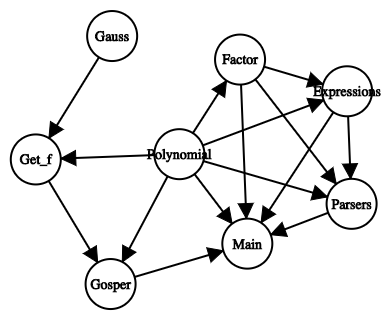
\includegraphics[width=0.6\textwidth]{images/dependency_graph.png}
\caption{Dependency graph of code}\label{Fig: DepGraph}
\end{figure}
Now that we have shown the general structure of the program, we will describe each of the important and interesting parts of the implementation. Firstly we will describe the structure used for parsing, thereafter we will discuss implementation of the methods needed for Wilf-Zeilberger's method. After that we will describe how a proof is written automatically and lastly we will shortly describe how testing has been done.

\section{Parsing}
In the project a several parsers are used. The parsers that have been implemented are shift-reduce parsers, which are a type of bottom-up parsers. In this type of parser a stack is used and a string is parsed character by character. When a character is read first the stack is reduced and then the character is pushed to the stack. That the stack is reduced means that if we read for instance a ''$+$'', then first all multiplications on the top of the stack are evaluated and first after that we push the ''$+$''. For more details and further explanation of a shift-reduce parser, see \reference{parser}.

In the code there are four parsers, which all read a string of a specific format and return either an object that the string represents or a string on another format. We are now going to describe the parsers with what they have as input and output, but first we need to describe an internal format that is used in the program to represent binomial coefficients, factorials and powers of integers. This format will in the rest of the report be referred to as \textit{the internal format} These three will be represented as follows:
\begin{center}
  \begin{tabular}{C{1mm}C{3cm}|C{4cm}|C{4cm}}
    &\textbf{What?}   & \textbf{Represented as:} & \textbf{Example:} \\ \hline
    &Factorial & $F[x]$, where $x$ is a polynomial & $(m+n)!$ is written as $F[n+m]$ \\ \hline
    &Binomial coefficient & $B[n,k]$ where $n,k$ are polynomials & $\binom{n+1}{k-1}$ is written as $B[n+1,k-1]$ \\ \hline
    &Power of integer & $P[a,n]$ where $a$ is an integer and $n$ is a polynomial & $2^n$ is written as $P[2,n]$ \\
  \end{tabular}
\end{center}

The parsers are described by the following table:
\begin{center}
  \begin{tabular}{C{1mm}C{3cm}|C{4cm}|C{4cm}}
    &\textbf{Parser}   & \textbf{Input format} & \textbf{Output format} \\ \hline
    &Polynomial parser & String with a polynomial, for instance ''n\^{}2+3km'' & Polynomial that the input string represents \\ \hline
    &Expression parser & String with an expression on the internal format, for instance ''(n!+k*m)/(n\^{}2+B[n,k])'' & Expression that the input string represents \\ \hline
    &\LaTeX parser     & String in \LaTeX format of an identity, for instance ''\textbackslash sum\_\{k=0\}\^{}n \textbackslash binom\{n\}\{k\}=2\^{}n'' & $F, a_k$ and the numerator and denominator of $\frac{a_k}{a_{k-1}}$ as the first step in the method \\ \hline
    &Internal format to \LaTeX parser  & String on the internal format & String on \LaTeX format \\
  \end{tabular}
\end{center}
\section{Gosper's algorithm}
Although the whole algorithm is described in section \ref{Sec: Gosper}, we will again go through the algorithm but from the perspective of implementation, and trying to point out difficulties along the way. There are some parts where the theory is straight forward, but the details in the implementation is quite difficult. In this section we try to describe the choices that were made during the work of the thesis, and also point out advantages and disadvantages with these choices.
\subsection{Finding p,q,r}
In section \ref{Sub: pqr} an algorithm is described for how to find polynomials $p,q,r$ such that
\begin{equation}\label{Eq: getpqr}
  \frac{a_k}{a_{k-1}} = \frac{p_k}{p_{k-1}}\frac{q_k}{r_k},
\end{equation}
such that $gcd(q_k,r_{k+j})=1 \forall j\geq 0$. The algorithm can be described as follows:
\begin{algorithm}[H]
  \caption{Get $p,q,r$}
  \inp{Rational polynomial $b=\frac{b_n}{b_d}=\frac{a_k}{a_{k-1}}$}
  \outp{Polynomials $p,q,r$ such that \ref{Eq: getpqr} holds and $gcd(q_k,r_{k+j})=1\forall j\geq 0$}
  \begin{algorithmic}[1]
    \Procedure{getpqr}{$b_n,b_d$}
      \State $r_k\gets b_d$
      \State $q_k\gets b_n$
      \State $p_k\gets 1$
      \While{$\exists j\geq 0: gcd(q_k,r_{k+j})\neq 1$}
        \State $j\gets \text{smallest } j \text{ such that } gcd(q_k,r_{k+j})\neq 1$
        \State $g_k\gets gcd(q_k,r_{k+j})$
        \State $q_k\gets \frac{q_k}{g_k}$
        \State $r_k\gets \frac{r_k}{g_{k-j}}$
        \State $p_k\gets p_kg_kg_{k-1}\ldots g_{k-j+1}$
      \EndWhile
      \State \Return $p_k,q_k,r_k$
    \EndProcedure
  \end{algorithmic}
\end{algorithm}
This algorithm is in theory fairly simple -- find a common factor and get rid of it -- but finding $gcd(q_k,r_{k+j})$ for all $j$ and see if this can be a common factor is tricky implementationwise. In the thesis this is implemented in the following fashion:
\begin{algorithm}[H]
  \caption{Find $GCD(q_k,r_{k+j})\forall j\geq 0$}
  \inp{Polynomials $q_k,r_k$}
  \outp{Polynomial $g_k=gcd(q_k,r_{k+j})$ for some $j\geq 0$}
  \begin{algorithmic}[1]
    \Procedure{GCDWithShift}{$q_k,r_k$}
      \State $g_{j,0}\gets r_k \text{ evaluated at } k=k+j$
      \State $g_{j,1}\gets \Call{GCD}{q_k,g_{j,0}}$
      \State $i\gets 1$
      \While{$g_{j,i}\neq 1$}
        \If{$\exists j^\prime\geq 0: g_{j,i}(j^\prime)=0$}\label{Alg: GCDWithShift,if}
          \State \Return $j^\prime$
        \EndIf
        \State $i\gets i+1$
        \State $g_{j,i}\gets \Call{GCD}{g_{j,i-2},g_{j,i-1}}$
      \EndWhile
      \State \Return $None$
    \EndProcedure
  \end{algorithmic}
\end{algorithm}
Here we perform the check in the if-statement on line \ref{Alg: GCDWithShift,if} by calling procedure \ref{Alg: Roots} and then checking if there is any root that is positive. Since this is the crucial step of this algorithm both the advantages and disadvantages come from the Roots-algorithm. In the implementation of Roots, only up to second degree polynomials are solved generally and after that values in the interval $(-100,100)$ are tested. This means that we cannot be sure that we find the roots. In general when we can use Wilf-Zeilberger's method, however, all roots are fairly small -- almost always less than 100. Therefore even though the implementation in theory is limiting it is very likely not to cause any problems in practice.
\subsection{Finding f}
The implementation in order to find the polynomial $f$ in Gosper's algorithm is performed just as described in section \ref{Sub: getf}. The goal of that is to find $f$ such that
\begin{equation}\label{Eq: getf}
  p_k=q_{k+1}f_k-r_kf_{k-1}.
\end{equation}
First the matrix $M$ and the vector $P$ are constructed. $M$ comes from the right hand side of \ref{Eq: getf} after assigning $f$ as stated in equation \ref{Eq: Theory,general polynomial}. $P$ is the vector that gives coefficients of the left hand side. After the construction Gaussian elimination is performed and then hopefully an answer will be given.

In case no answer has been found one can try to increase the maximal degree of $f$. It is not certain however that a solution can be given by this method since possibly the degree of the smallest degree solution for $f$ can be arbitrarily large with respect to the variables that are not $k$. If this can be the case has not neither been proved or disproved. If a solution is given, however, then we have performed the whole Gosper's algorithm.
\section{Proof generation}
The proof generation is a method which needs an input string and a parser. Then the method produces a proof, written in \LaTeX code, for that the input string in fact is true. Right now the parser that has been developed in the thesis can only handle a few different types of operators in the input string -- binomial coefficients, factorials, integer powers and polynomials can be handled, but no other operators. The reason for this is that the parser mostly is an example of how Wilf-Zeilberger's method can be used, and is not meant to be a full solution. Instead users can write their own parsers and input strings which convert the string into four things: $F,a_k$ and the numerator and denominator of the fraction $\frac{a_k}{a_{k-1}}$. When the user has provided this parser and input string, then the main-function does the rest of the job in producing the proof in \LaTeX format, which proves the identity.

The reasons for this design choice (to only provide a simple parser as an example) are a few: firstly this gives a flexibility for a user and works well in an open source setting, secondly it would be at least as time demanding as writing the rest of the method to write a more general parser for more kinds of identity parsing -- and still some applications would probably be left out anyways.

The general methodology used in the proof generation is the following:
\begin{enumerate}[i)]
  \item Get a parser and an input string as inputs.
  \item Parse the string, which gives us $F,a_k$ and the polynomials that are the numerator and denominator of $\frac{a_k}{a_{k-1}}$.
  \item Call Gosper's algorithm which gives a $G(n,k)$ such that $G(n,k+1)-G(n,k)=a_k=F(n+1,k)-F(n,k)$. This step is the main contribution from the program, and is usually the by far hardest part of the proof.
  \item Write the proof in \LaTeX format.
  \item Highlight parts of the proof that need to be verified or partly proved by the user. This includes proving that $\lim_{k\to\pm\infty}G(n,k)=0\forall n$ and may include verifying that $G(n,k+1)-G(n,k)=F(n+1,k)-F(n,k)$. This should be guaranteed by the solver, but might be worth verifying.
\end{enumerate}
\section{Testing}
In general the testing has tried to test each method individually and then first after each methods works on its own it has been tested all together. The testing on each individual method has been performed in different ways for different methods, but the common thing for all of the methods is that the testing included many edge cases as well as other cases. Edge cases are usually when some parameters (for instance the degree of a polynomial or the number of variables in the polynomial) is very small or large.

The tests that were performed on methods all together are usually from one of the test examples provided in chapter \ref{Ch: Results}. Then the implementation and testing was iterated until all identities worked. This testing was also performed in steps, for instance in order to test the methods in Gosper's algorithm, some initial steps were done by hand and then the relevant part was tested. Then, when all individual methods and groups of methods worked as expected, everything was put together and the final result was given.


\chapter{Results}\label{Ch: Results}
Throughout the thesis some identities have been used for testing the code, these will be called training examples. All identities that have been used in this thesis have been collected from \reference{gould}, \reference{bucht} and \reference{tesler}. When choosing the training examples many identities were considered and we tried to find a good variety of identities, both well known and not as well known ones as well as using identities that look quite different. The identities used as training examples are the following:
\begin{enumerate}
  \item $\sum_{k=0}^n \binom{n}{k} = 2^n$ \label{ID: 1}
  \item $\sum_{k=0}^n (-1)^k\binom{n}{k}\binom{2k}{k}4^{n-k}=\binom{2n}{n}$ \label{ID: 2}
  \item $\sum_{k=0}^n \binom{n}{k}^2 = \binom{2n}{n}$ \label{ID: 3}
  \item $\sum_{k=0}^n 2^k\binom{n}{k} = 3^n$ \label{ID: 4}
  \item $\sum_{k=0}^n k\binom{n}{k} = n2^{n-1}$ \label{ID: 5}
  \item $\sum_{k=1}^n \frac{1}{k(k-1)} = 1-\frac{1}{n}$ \label{ID: 6}
  \item $\sum_{k=0}^n \binom{k}{c} = \binom{n+1}{c+1}$ \label{ID: 7}
  \item $\sum_{k=0}^n \binom{r+k}{k} = \binom{r+n+1}{n}$ \label{ID: 8}
  \item $\sum_{k=0}^n \binom{m-k}{n-k} = \binom{m+1}{n}$ \label{ID: 9}
  \item $\sum_{k=n}^\infty \frac{1}{\binom{k}{n}}=\frac{n}{n-1}$ \label{ID: 10}
\end{enumerate}
Some of these identities are quite trivial to show with combinatorial arguments, but others are not as easy. For instance identity \ref{ID: 1} comes from counting in how many ways we can choose objects out of $n$ different objects, while identity \ref{ID: 2} is not very easy to prove by providing a combinatorial argument. When these identities are shown, a \LaTeX file is produced. The proofs of all identities are provided in chapter \ref{Ch: Attachments}. As we can see the identities \ref{ID: 7} and \ref{ID: 8} cannot be shown, the reason for this is that the ''get f'' method cannot give a solution, since $f$ cannot be a polynomial. This is because the degree of $f$ depends on $c$ and $r$, respectively, and therefore \WZ does not work well on the problem.

After the program worked for all the training examples the program was validated on other identities (called validation examples), in the hopes that the program works on identities it has not been developed to work on as well. Also here we tried to use validation identities that are different from each other, but now we also prioritized identities that are not very simple to solve with combinatorial arguments. The tests that were used are:
\begin{enumerate}
  \setcounter{enumi}{10}
  \item $\sum_{k=0}^n 3^k\binom{n}{k} = 4^n$ \label{ID: 11}
  \item $\sum_{k=0}^n 4^k\binom{n}{k} = 5^n$ \label{ID: 12}
  \item $\sum_{k=0}^n \binom{n}{2k} = 2^{n-1}$ \label{ID: 13}
  \item $\sum \frac{1}{k\binom{k+n}{k}} = \frac{1}{n}$ \label{ID: 14}
  \item $\sum_{k=0}^\infty 2^{-k}\binom{n+k}{k} = 2^{n+1}$ \label{ID: 15}
  \item $\sum_{k=0}^n \frac{\binom{n}{k}}{\binom{2n-1}{k}} = 2$ \label{ID: 16}
  \item $\sum_{k=0}^n k\frac{\binom{n}{k}}{\binom{2n-1}{k}} = 2\frac{n}{n+1}$ \label{ID: 17}
  \item $\sum_{k=1}^{2n-1} (-1)^{k-1}\frac{k}{\binom{2n}{k}} = \frac{n}{n+1}$ \label{ID: 18}
  \item $\sum_{k=0}^n \binom{2n+1}{k} = 2^{2n}$ \label{ID: 19}
  \item $\sum_{k=0}^{\frac{n}{2}} (-1)^k\binom{n-k}{k}\frac{2^{2n-2k}}{n-k} = \frac{2^{n+1}}{n}$ \label{ID: 20}
\end{enumerate}
As we can see in chapter \ref{Ch: Attachments} the program manages to solve most of the validation examples. The program solves identities \ref{ID: 11}, \ref{ID: 12}, \ref{ID: 14} and \ref{ID: 15} perfectly. For identities \ref{ID: 16} and \ref{ID: 17} the program manages to get a $G$ which works in \WZ but has not been able to verify that the first condition for a certifying pair is fulfilled. This has been done by hand afterwards though. For identity \ref{ID: 13} the program does not manage to prove the identity, this is since it cannot find a $f$ that works. The reason for this is that the difference in degrees cannot be resolved on the right and left side when getting $f$. Therefore \WZ cannot be used to solve this identity.


\chapter{Discussion and conclusions}\label{Ch: Discussion and conclusions}
In the thesis \WZ has been implemented with a library of polynomials as a foundation. During the work on the thesis it has become more and more obvious how even the simplest operations in theory might be quite tricky to implement with computer algebra. Furthermore it became brutally clear how details in program design could help or harm the rest of the dependent parts of the program. This required more thought before implementation, and also better code in general.

The program seems to work fine but has some obvious limitations. First of all only a very small part of all proofs can be shown by \WZ, and as we saw in chapter \ref{Ch: Results} two seemingly similar identities, for instance identities \ref{ID: 7} and \ref{ID: 9}, can have two very different outcomes when trying to use \WZ -- one is solvable and one is not! This makes it harder to trust the method to solve a problem that is given.

Secondly the method needs to have an identity to prove. \WZ itself cannot come up with a guess for what a sum is, but only prove the correctness or incorrectness of an identity once it is already guessed.

Thirdly with the current state of the implementation it is not obvious which part of the method that fails. Usually it is the part where we try to find polynomial $f$ such that $p_k=q_{k+1}f_k-r_kf_{k-1}$, but it can also be other problems that make the program fail. Also when trying to find polynomial $f$, it is not certain what causes the problem. It can be both that the degree of the assigned polynomial is too small, and that the problem in fact is not solvable for some reasons.

Lastly, the \WZ solver that has been developed leaves a few parts of the formal proof for the user to show. This is not optimal, however showing these parts automatically as well would demand even more implementation and was out of scope for this thesis.

Still, even though there are clear problems with both the \WZ itself and the implementation that was chosen, we would like to argue that the thesis has value and contributes to the general knowledge about infinite sumation. If one has an identity it can quickly be checked if it is possible for the \WZ solver to prove it. If it can, then one quickly have a proof and otherwise other methods have to be used. Even though it is not directly obvious what goes wrong when the solver fails to prove an identity, the implementation is split up in many different methods, which makes is fairly easy to get a sense of what goes wrong.

From the examples that were tested we can conclude that \todo[inline]{continue}

The problem that \WZ cannot guess what a sum equals is a problem for the whole method. Finding ways to guess what a sum equals is also a very interesting area that would be fun to explore more, but is out of score for this thesis.


\begin{thebibliography}{99}
\bibitem{veltman}Veltman, M.J.G. and Williams, D.N. (1991). 'Schoonschip ’91.'\label{Ref: veltman}
\bibitem{maple}Lopez, R. \textit{Computer Algebra Systems.} Maplesoft, viewed 26 November 2019. \url{https://www.maplesoft.com/ns/maple/cas/computer-algebra-systems-math-education.aspx}.\label{Ref: maple}
\bibitem{computeralgebra}Güyer, T. (2008). 'Computer Algebra Systems as the Mathematics Teaching Tool.' \textit{World Applied Sciences Journal} 3 (1): 132-139, 2008.\label{Ref: computeralgebra}
\bibitem{wz}Wilf, H.S., and Zeilberger, D. (1990). 'Rational functions certify combinatorial identities.' \textit{J. Amer. Math. Soc. 3} (1990), pp. 147–158.\label{Ref: wz}
\bibitem{mathematica}Paule, P. and Schorn, M. (1994). 'A Mathematica Version of Zeilberger's Algorithm for Proving Binomial Coefficient Identities.' \textit{J. Symbolic Computation} (1995) 20, pp. 673--698.\label{Ref: mathematica}
\bibitem{wilf}Wilf, H.S. (1994). \textit{Generating functionology.} Academic Press, Inc. Philadelphia, Pennsylvania.\label{Ref: wilf}
\bibitem{gosper}Gosper, R.W. Jr. (1978). \textit{Decision procedure for indefinite hypergeometric summation.} Proc. Natl. Acad. Sci. USA. Vol. 75, No. 1, pp. 40--42, January 1978. Palo Alto, California.\label{Ref: gosper}
\bibitem{parser}Johnson, M. (2007). \textit{Handout 08 Bottom-up Parsing.} Lecture notes Stanford University CS143. Delivered 2 July 2007. \url{https://web.archive.org/web/20160305041504/http://dragonbook.stanford.edu/lecture-notes/Stanford-CS143/08-Bottom-Up-Parsing.pdf}\label{Ref: parser}
\bibitem{gould}Gould, H.W. (1972). \textit{Combinatorial Identities.} Morgamtown Printing and Binding Co. West Virginia.\label{Ref: gould}
\bibitem{tesler}Tesler (2017). \textit{Chapter 3.3, 4.1, 4.3. Binomial Coefficient Identities.} Lecture notes University of California San Diego Math 184A. Delivered winter 2019. \url{http://www.math.ucsd.edu/~gptesler/184a/slides/184a_ch4slides_19-handout.pdf}\label{Ref: tesler}

\end{thebibliography}

\chapter{Attachments}\label{Ch: Attachments}
\section{Code}
All code is available on \url{https://github.com/LarsAstrom/Wilf-Zeilbergers-Method/tree/master/WZmethod}.
\section{Proofs of identities}
We want to remind the reader that in Wilf-Zeilberger's method we find a polynomial $F(n,k)$. Then we want to find another polynomial $G$ such that $(F,G)$ is a certifying pair of polynomials, meaning that
\begin{enumerate}
  \item $F(n+1,k)-F(n,k)=G(n,k+1)-G(n,k)$, and
  \item $\lim_{k\to\pm\infty} G(n,k)=0, \forall n$.
\end{enumerate}
We can also express this by finding a proof certificate $R(n,k)$ such that
\begin{equation*}
  G(n,k)=R(n,k)F(n,k-1).
\end{equation*}
\proofimage{images/proof01.png}{Proof of identity \ref{ID: 1}.}
\proofimage{images/proof02.png}{Proof of identity \ref{ID: 2}.}
\proofimage{images/proof03.png}{Proof of identity \ref{ID: 3}.}
\proofimage{images/proof04.png}{Proof of identity \ref{ID: 4}.}
\proofimage{images/proof05.png}{Proof of identity \ref{ID: 5}.}
\proofimage{images/proof06.png}{Proof of identity \ref{ID: 6}.}
\proofimage{images/proof07.png}{Proof of identity \ref{ID: 7}.}
In both proof 7 and 8 we have integer variables, $c$ and $r$ respectively. These cause problems in step 2 in Gosper's algorithm, since the polynomial $f$ would have a degree dependent on $c$ and $r$, respectively. This cannot be handled by the automatic solver.
\proofimage{images/proof08.png}{Proof of identity \ref{ID: 8}.}
\proofimage{images/proof09.png}{Proof of identity \ref{ID: 9}.}
\proofimage{images/proof10.png}{Proof of identity \ref{ID: 10}.}
\proofimage{images/proof11.png}{Validation of program. Proof of identity \ref{ID: 11}.}
\proofimage{images/proof12.png}{Validation of program. Proof of identity \ref{ID: 12}.}
\proofimage{images/proof13.png}{Validation of program. Proof of identity \ref{ID: 13}.}
The automatic prover cannot find a polynomial $f$ in step 2 of Gosper's algorithm. This is since the degree (with respect to $n$) of the left and right hand side of the equation
\begin{equation}
  p_k=q_{k+1}f_k-r_kf_{k-1}
\end{equation}
cannot be the same.
\proofimage{images/proof14.png}{Validation of program. Proof of identity \ref{ID: 14}.}
\proofimage{images/proof15.png}{Validation of program. Proof of identity \ref{ID: 15}.}
\proofimage{images/proof16.png}{Validation of program. Proof of identity \ref{ID: 16}.}
\proofimage{images/proof17.png}{Validation of program. Proof of identity \ref{ID: 17}.}
\proofimage{images/proof18.png}{Validation of program. Proof of identity \ref{ID: 18}.}
Also in this example the automatic solver cannot prove the identity, and the problem lies in step 2 of Gosper's algorithm.
\proofimage{images/proof19.png}{Validation of program. Proof of identity \ref{ID: 19}.}
\proofimage{images/proof20.png}{Validation of program. Proof of identity \ref{ID: 20}.}
\newpage
\section{Popular Scientific Paper}
\pagestyle{empty}
\popimage{images/pop_v1_2.png}



\end{document}
